\section{Problem formulation}
\label{sec:problem-formulation}
In this section, an outline of the system model describes servers and tasks attributes
(subsection~\ref{subsec:system-model}) used in the resource elastic optimisation problem
(subsection~\ref{subsec:optimisation-problem}). Using this model, we prove that it is NP-Hard
(subsection~\ref{subsec:time-complexity}). Finally, using a example program, we demonstrate in the effectiveness of our
flexible resource allocation scheme compared to an fixed resource allocation scheme used in previous work, as explained
the previous section (subsection~\ref{subsec:example-problem-case}).

\subsection{System model}\label{subsec:system-model}
\begin{wrapfigure}{r}{0.4\linewidth}
    \centering
    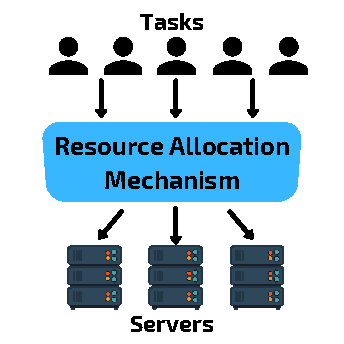
\includegraphics[width=\linewidth]{figs/system_model.pdf}
    \caption{System Model}
    \label{fig:system-model}
\end{wrapfigure}
A sketch of the system is shown in Fig.~\ref{fig:system-model}.
We assume that there are a set of servers $I = \{1,2,\ldots,\left|I\right|\}$, which could be accessed either through
cellular base stations or WiFi access points (APs). These servers have different types of limited resources:
storage for the code/data needed to run a task (e.g., measured in Gb), computation capacity in terms of CPU cycles per
time interval (e.g., measured in Ghz), and communication bandwidth to receive the data and to send back the results
of the task after execution per time interval (e.g., measured in Mbit). The servers are assumed to only consider these
attributes for resource allocation, however future work would wish to explore additional attributes like I/O memory
access per second, GPU usage, and more. The servers are also assumed to be heterogeneous in all their characteristics.
Formally, we denote the storage capacity of server $i$ with $S_i$, the computation capacity with $W_i$, and the
bandwidth capacity with $R_i$.

The system also contains a set $J = \{1,2,\ldots,\left| J \right|\}$, of different tasks that each require service from
one of the servers $I$. Each task has a monetary value, denoted $v_j$, representing the maximum price the owner is
willing to pay for the task to be computed. \\
In order to run a task, the server is required to load the appropriate code/data onto the server from a source, then to
compute the code of the task and to send back results to the user. Therefore, for each of these stages, we consider
separate speeds that the operations could occur at to enable the greatest flexibility for the server at each stage. \\
The storage size for the task $j$ is denoted as $s_j$ with the rate that the program is transferred to the server
as $s^{'}_j$. For a task to be computed successfully, it must fetch and execute instructions on a CPU. We consider the
total number of CPU cycles required for the program to be $w_j$, where the number of CPU cycles assigned to the task
per unit of time as $w^{'}_j$. Finally, after the task is run and the results obtained, the latter need to be sent back
to the user. The size of the results for task $j$ is denoted with $r_j$, and the bandwidth used to sent back results to
the user as $r^{'}_j$.

In order to force the server to complete the task with a reasonable time, each task sets a deadline, denoted by $d_j$,
representing the maximum amount of time for a task to be completed successfully within. This includes: the time
required to load the data/code onto the server, run it, and send back results to the user. We assume that there
is an \emph{all}-or-\emph{nothing} task execution reward scheme, meaning that the task value is awarded only if the
task is completed within its deadline.

\subsection{Optimisation problem}
\label{subsec:optimisation-problem}
Given the aforementioned assumptions and variables from the system model, an optimisation problem is constructed as
followed. This problem uses the additional variable $x_{i,j}$ to denote the allocation of a task $j$ that will run on
server $i$.

\begin{align}
    \max & \sum_{\forall j \in J} v_j \left(\sum_{\forall i \in I} x_{i,j}\right) \label{eq:objective} \\
    \mbox{s.t.} \nonumber \\
    & \sum_{\forall j \in J} s_j x_{i,j} \leq S_i, &~ \forall{i \in I} \label{eq:server-storage-constraint} \\
    & \sum_{\forall j \in J} w^{'}_j x_{i,j} \leq W_i, &~ \forall{i \in I} \label{eq:server-computation-constraint} \\
    & \sum_{\forall j \in J} (r^{'}_j + s^{'}_j) \cdot x_{i,j} \leq R_i, &~ \forall{i \in I} \label{eq:server-bandwidth-constraint} \\
    & \frac{s_j}{s^{'}_j} + \frac{w_j}{w^{'}_j} + \frac{r_j}{r^{'}_j} \leq d_j, &~ \forall{j \in J} \label{eq:task-deadline} \\
    & 0 < s^{'}_j, &~ \forall{j \in J} \label{eq:loading-speeds} \\
    & 0 < w^{'}_j, &~ \forall{j \in J} \label{eq:compute-speeds} \\
    & 0 < r^{'}_j, &~ \forall{j \in J} \label{eq:sending-speeds} \\
    & \sum_{\forall i \in I} x_{i,j} \leq 1, &~ \forall{j \in J} \label{eq:server-task-allocation} \\
    & x_{i,j} \in \{0, 1\}, &~ \forall{i \in I},\forall{j \in J} \label{eq:task-allocation}
\end{align}

The objective (eq.~\ref{eq:objective}) is to maximize the total value over all tasks (i.e.,\ social welfare) that
are completed within their deadline (eq.~\ref{eq:task-deadline}).
Constraints~\ref{eq:server-storage-constraint},~\ref{eq:server-computation-constraint}
and~\ref{eq:server-bandwidth-constraint}, prevent over allocation of server resources to allocated tasks.
For the server's storage capacity (constraint~\ref{eq:server-storage-constraint}), each server's storage must be less
than the allocated task's storage requirements. While for the server's computational capacity
(constraint~\ref{eq:server-computation-constraint}), the capacity is limited by a server's allocated tasks
compute resources ($w^{'}_j$). The server's bandwidth capacity (constraint~\ref{eq:server-bandwidth-constraint})
comprises of two parts: the first for loading of data/code of a task onto the server and the second for sending
back result to the user. \\
To force the task to the completed within its assigned deadline, constraint~\ref{eq:task-deadline} required the sum
of time taken for each stages of the task, completed in series, to be less than the deadline value.
Note that if a task is not allocated to any server, this constraints can be satisfied by choosing arbitrarily
resource speed as these resources do not use up any servers' resources in
constraint~\ref{eq:server-storage-constraint},~\ref{eq:server-computation-constraint}
or~\ref{eq:server-bandwidth-constraint}. \\
Constraints~\ref{eq:loading-speeds},~\ref{eq:compute-speeds},~\ref{eq:sending-speeds} enforce that the resource
speeds for each stage ($s^{'}_j$, $w^{'}_j$, and $r^{'}_j$) are all positive and finite.
Finally, as every task can only be served by at most one server, constraints~\ref{eq:server-task-allocation}
and~\ref{eq:task-allocation} enforce this.

This model focus on a single-shot setting where all tasks arrival at the same time to the system. To use this system
in practice where tasks arrival progressively over time, an allocation mechanism would repeat the allocation decisions
described here over regular time intervals. As a result, longer running tasks would reappearing in consecutive time
intervals.
In subsection~\ref{subsec:comparison-between-online-and-batched-resource-allocation}, we evaluate the effectiveness of
such a batching mechanism compared to online mechanisms. We leave a detailed study of online mechanisms to future work.
A probably advantage of such a system is the ability to dynamically change the resource allocation at each time step.

\subsection{Time Complexity}
\label{subsec:time-complexity}
As the optimisation problem as described in Subsection~\ref{subsec:optimisation-problem} is an extension of the
Knapsack problem, a well-studied problem in computer science that known to be NP-Hard. By transforming the problem into
a standard knapsack problem, the time complexity of the problem is also NP-Hard.
\begin{theorem}
    The optimisation problem in subsection~\ref{subsec:optimisation-problem} is NP-hard.
\end{theorem}
\begin{proof}
    The task resource elasticity~\ref{eq:task-deadline} can removed from the optimisation problem to simplify the model
    by setting the task resource speeds to a fixed value that satisfies the deadline constraint. This reduces the model
    to a 0--1 multidimensional knapsack problem~\cite{knapsackproblems_2004}, which is a generalization of a
    simple 0--1 knapsack problem. The latter is an NP-hard problem~\cite{knapsackproblems_2004}. Given this, it follows
    that the 0--1 multidimensional knapsack problem is also NP-hard. Since the optimization problem
    (Eqs.~\ref{eq:objective} -~\ref{eq:task-allocation}) is a generalization of a 0--1 multidimensional knapsack
    problem, it follows that it is NP-hard as well.
\end{proof}

\subsection{Example Problem Case}
\label{subsec:example-problem-case}
\begin{wrapfigure}{l}{0.5\linewidth}
    \centering
    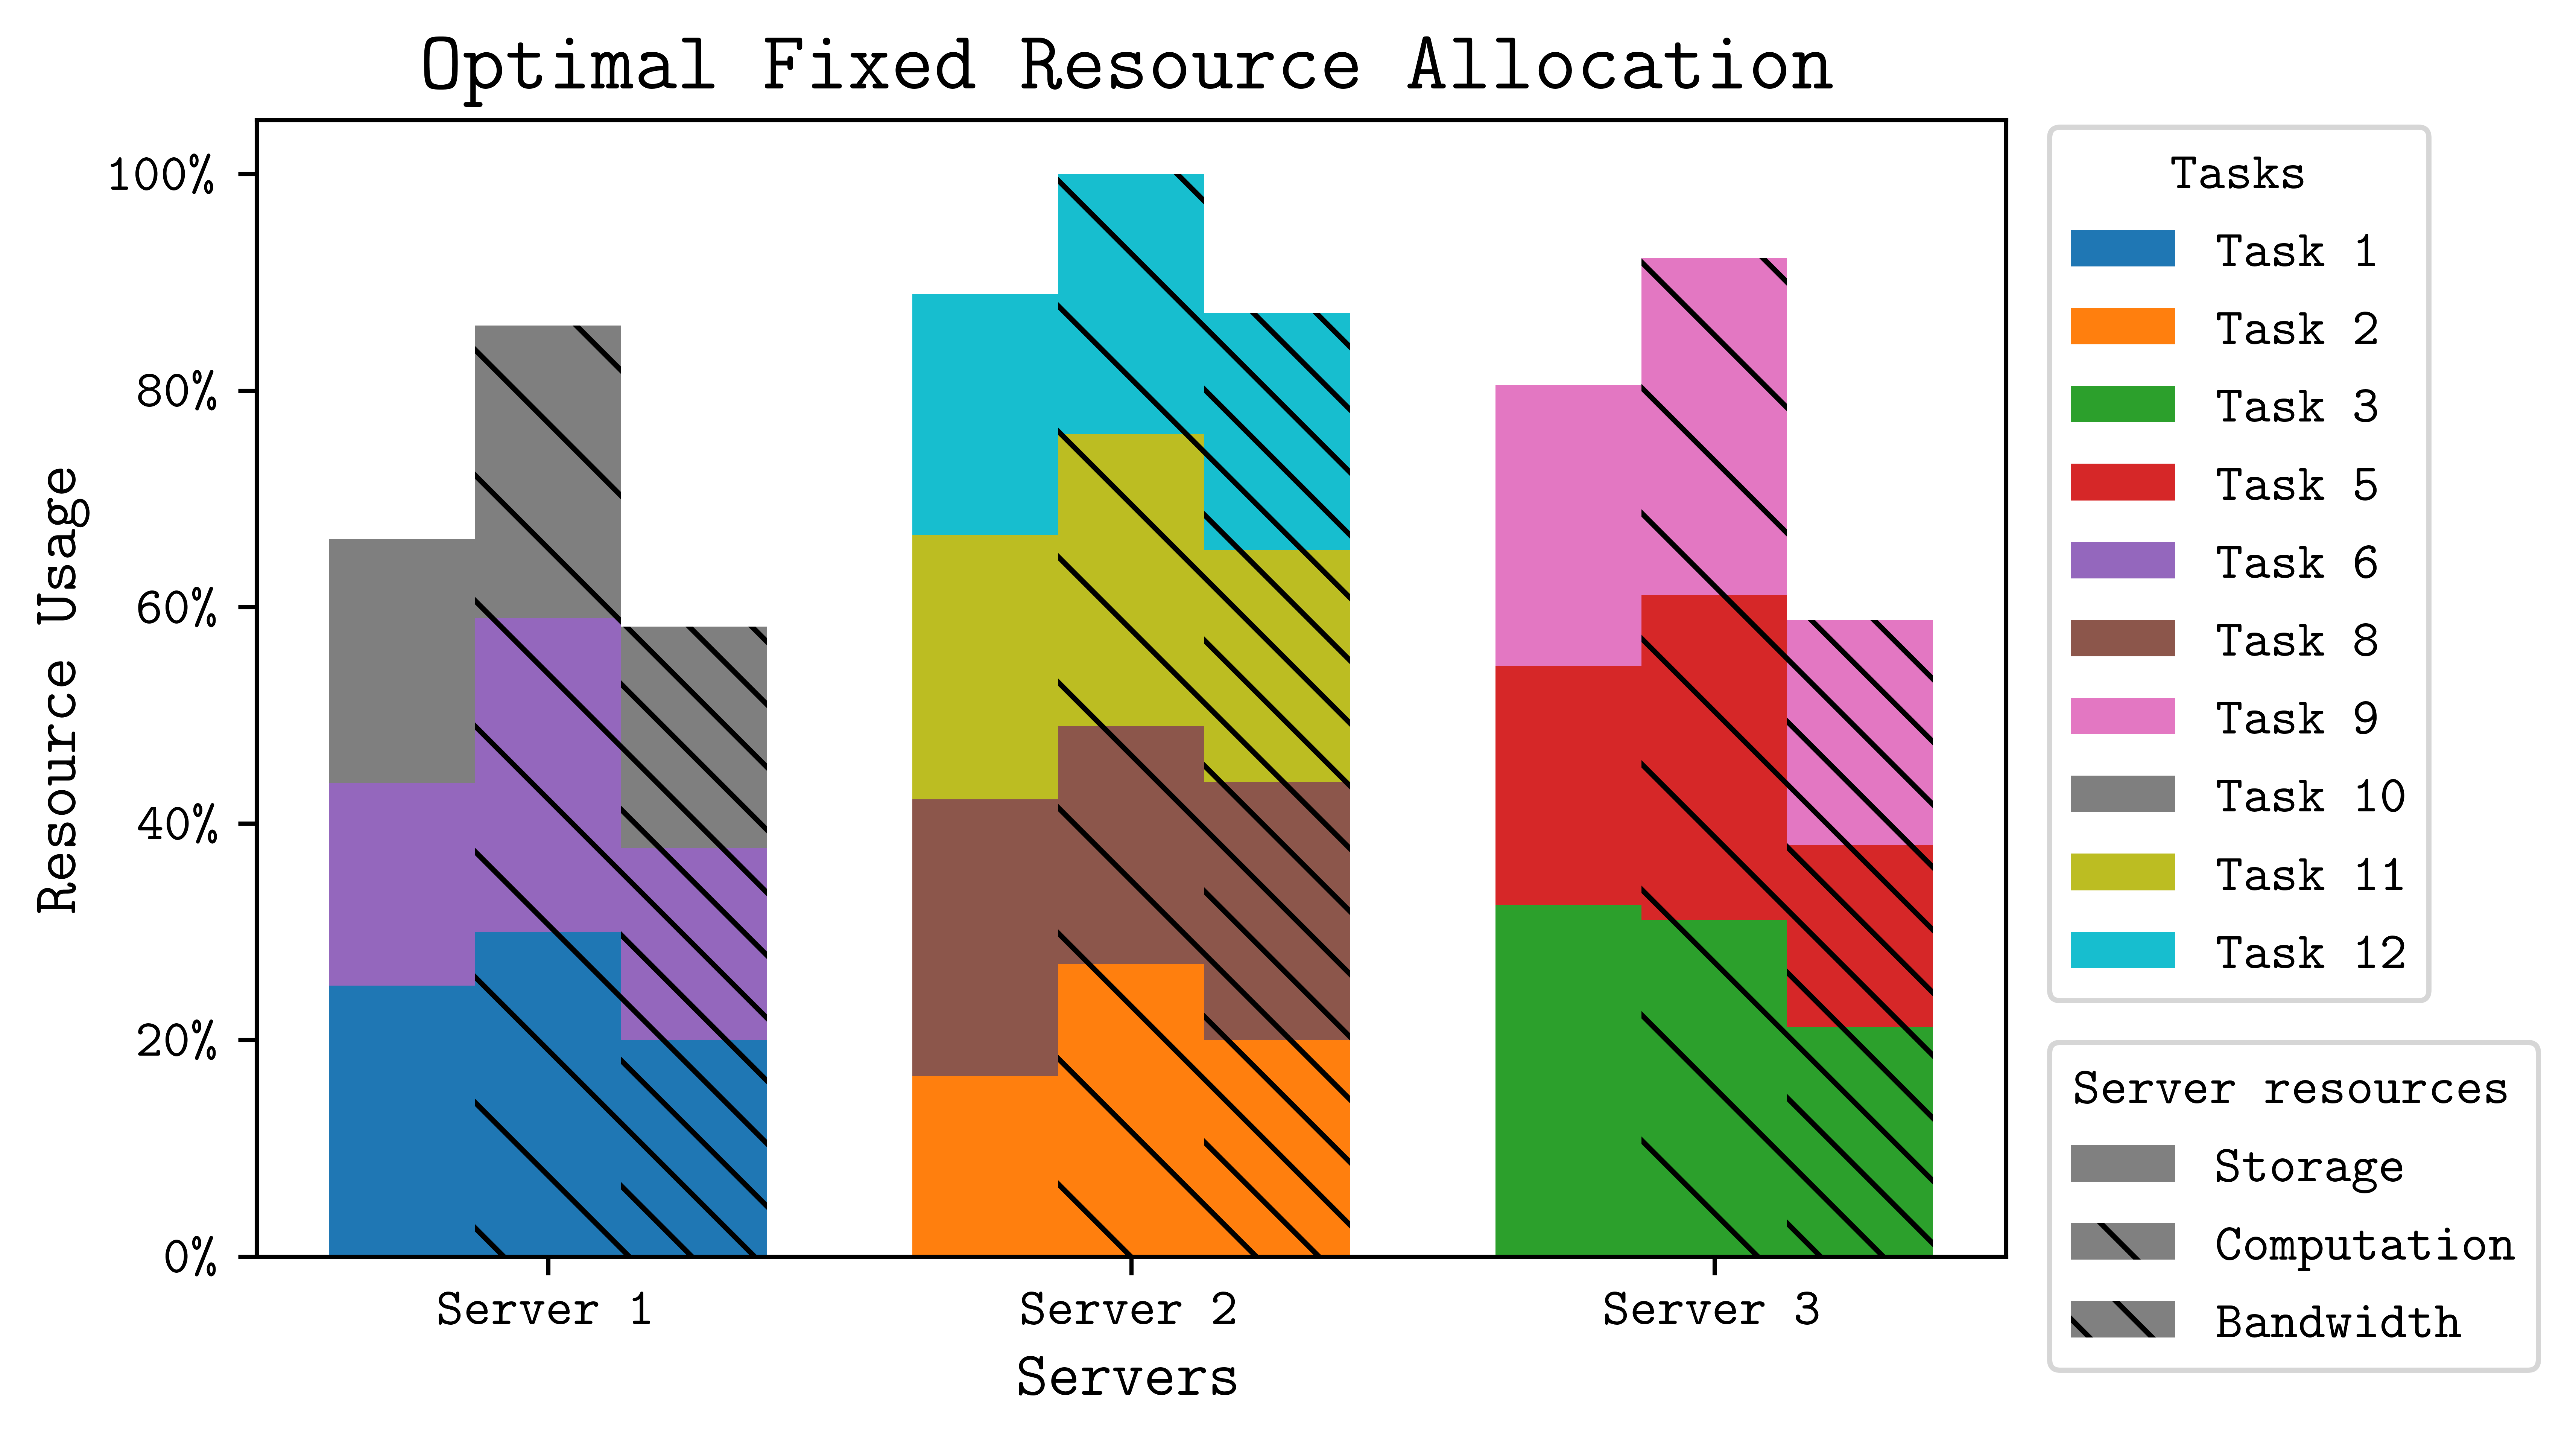
\includegraphics[width=\linewidth]{figs/allocation/optimal_fixed_resource_allocation.png}
    \caption{Optimal solution with fixed resource speeds}
    \label{fig:example-fixed-allocation}
\end{wrapfigure}
Before we propose our allocation mechanisms in the next section, we present an example case to illustrate
why elasticity is important. In this example, there are 12 potential tasks and 3 servers where the flexible solution
is able to achieve 18\% better social welfare compared to the fixed resource allocation solution.
The exact settings can be found in Appendix A with table~\ref{tab:example-tasks-properties}
for the task attributes and table~\ref{tab:example-servers-properties} for the server attributes. \\
The figures~\ref{fig:example-fixed-allocation} and~\ref{fig:example-flexible-allocation} represent each server as a
group of three bars, each relating to each server's resource type, with the percentage of resources used by a task
being the size of the bar.

\begin{figure}
    \centering
    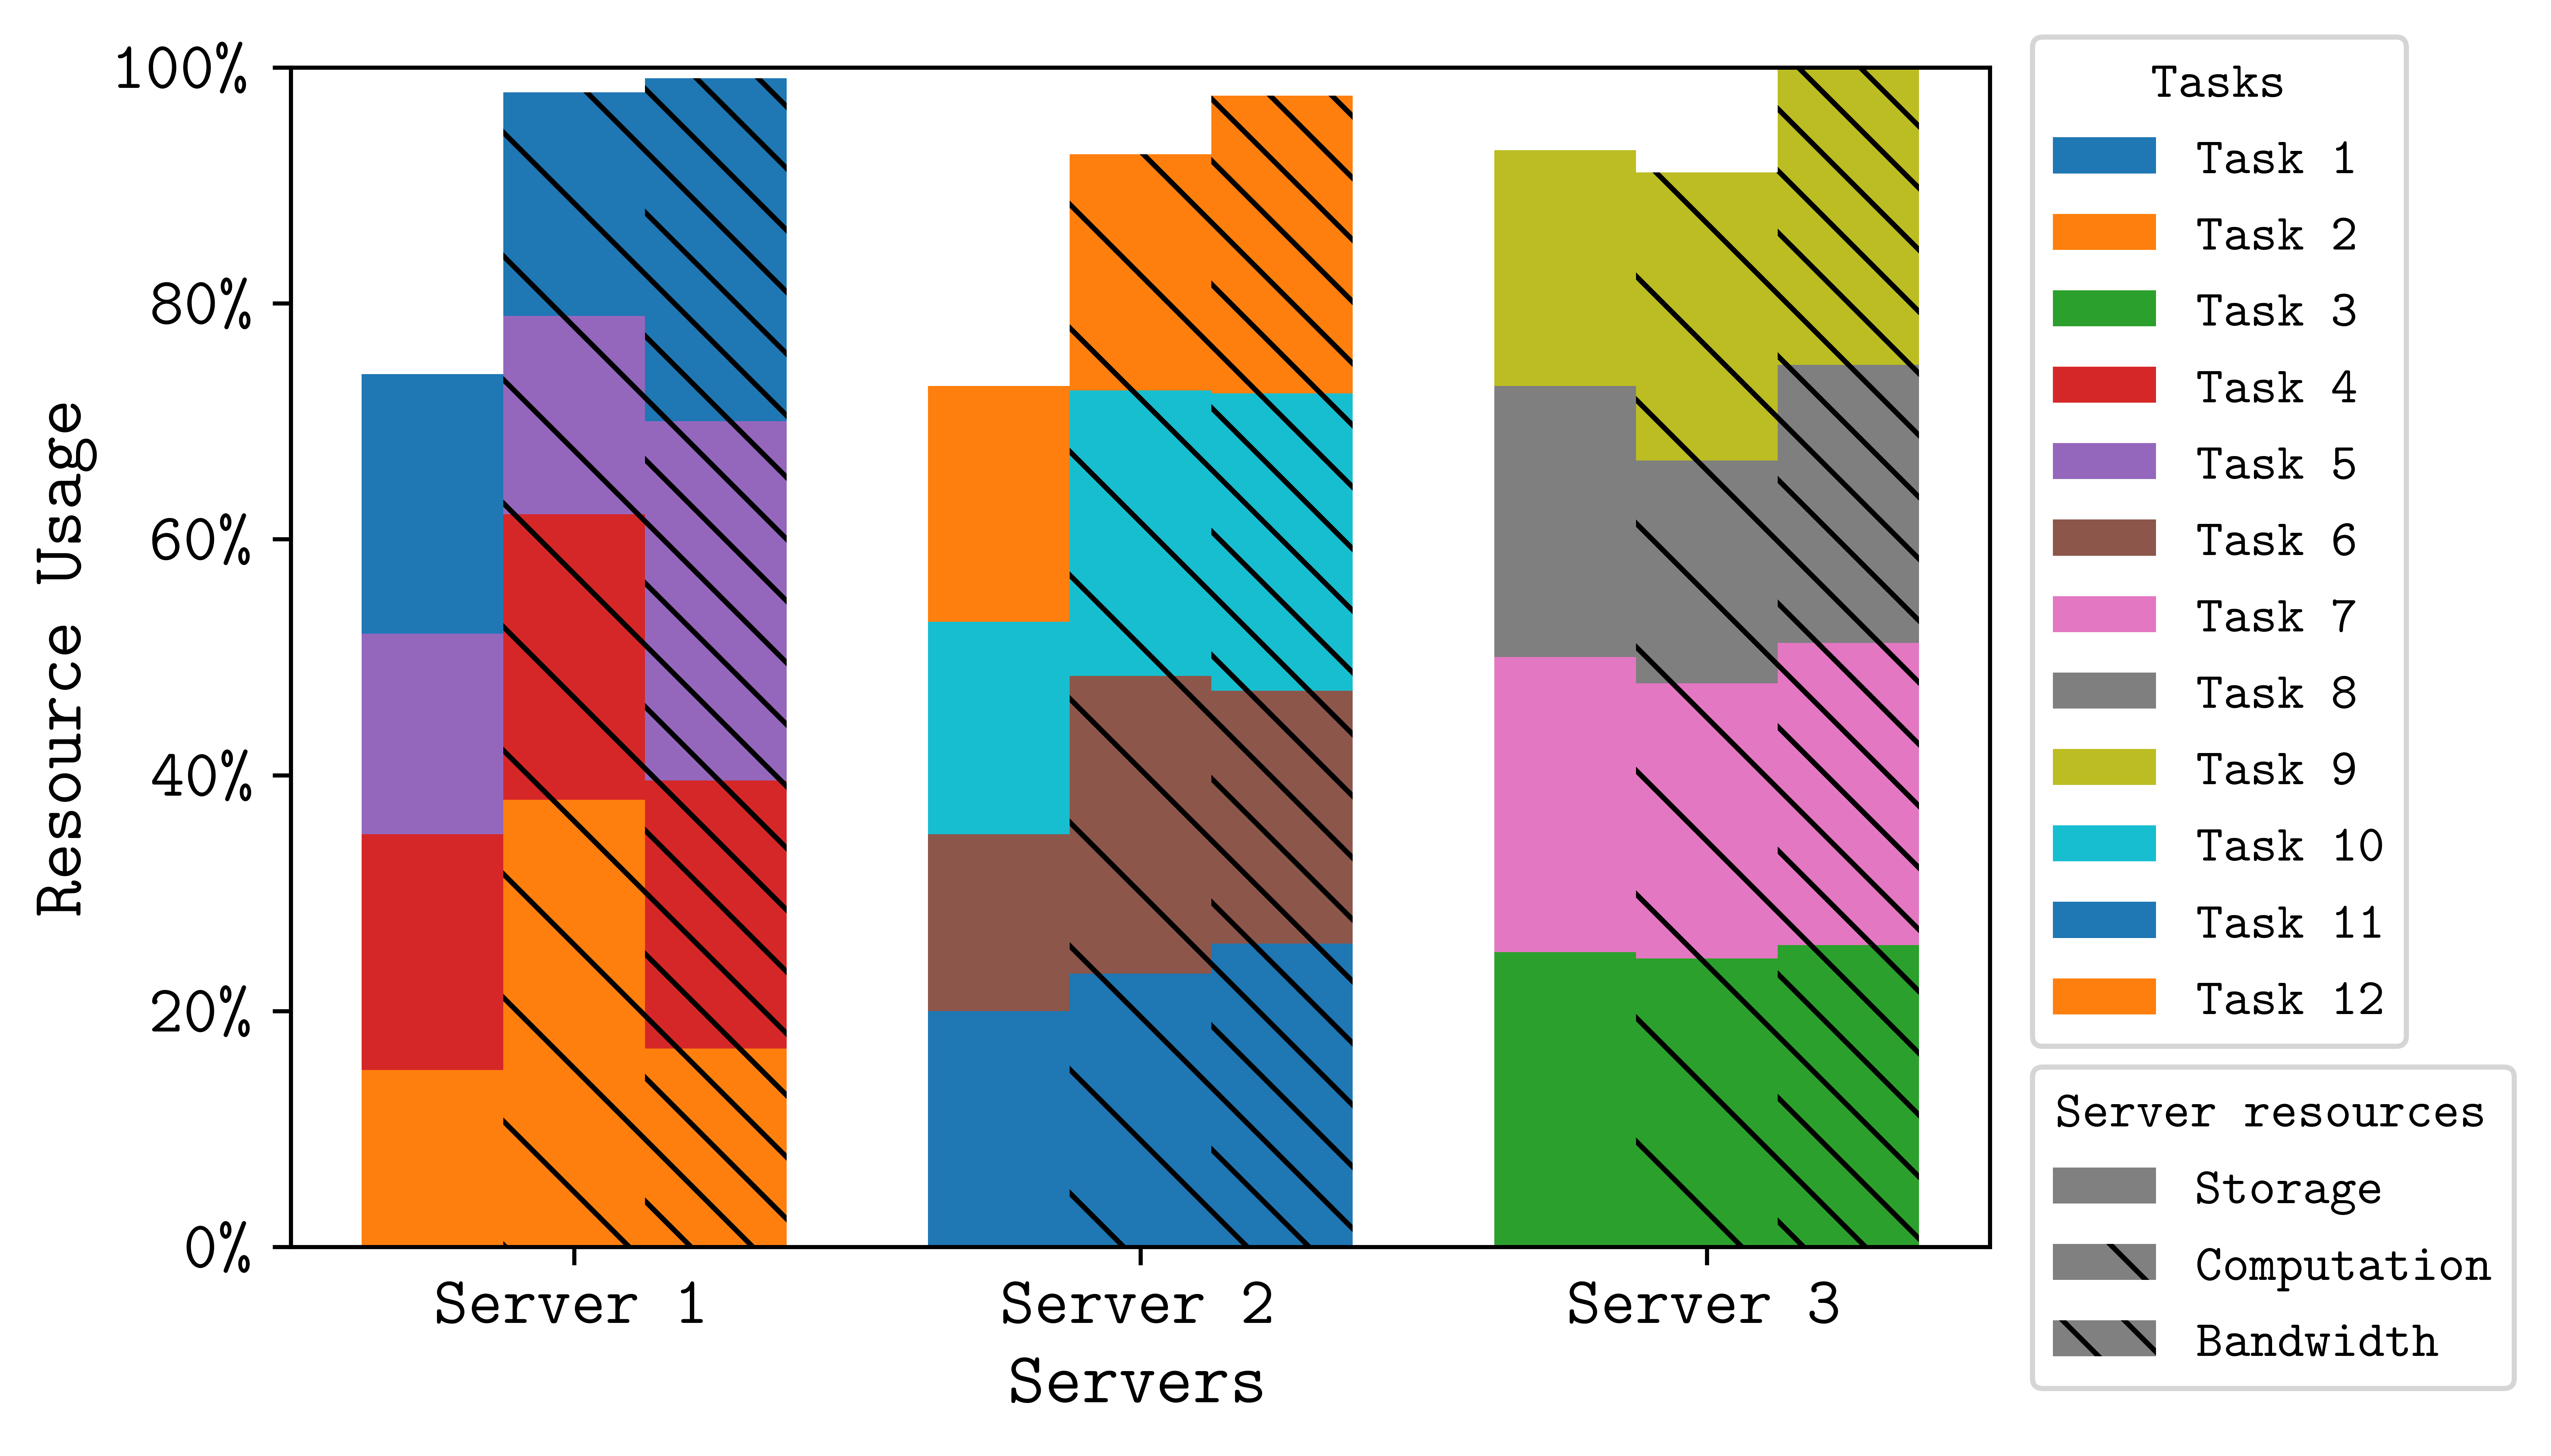
\includegraphics[width=0.5\linewidth]{figs/allocation/optimal_flexible_resource_allocation.png}
    \caption{Optimal solution with elastic resources speeds}
    \label{fig:example-flexible-allocation}
\end{figure}

Figure~\ref{fig:example-fixed-allocation} shows the best possible allocation if tasks have fixed resource speeds (which
were set by minimising the total amount of resources to be completed within the deadline). Here, only 9 of the tasks
are run, resulting in a total social welfare of 980 due to server 1 and 2's limited computational capacity and server
3' limited communication capacity.

In contrast to figure~\ref{fig:example-fixed-allocation}, Figure~\ref{fig:example-flexible-allocation} depicts the
optimal allocation if elastic resources are considered. Here, all the resources are used by the servers, whereas the
fixed example~\ref{fig:example-fixed-allocation} cant do this. In total, the elastic approach manages to schedule all
12 tasks within the resource constraints, achieving a total social welfare of 1200 (an 18\% improvement over the fixed
approach).